\documentclass[12pt,a4paper]{article}
% Toan_11_04.tex - Bien soan lai noi dung PDF: FILE chuyen dung TDM11X14
% Trinh bay theo phong cach BTVN_Luong_giac_01_B1.tex (toan_11).
% Tai lieu doc lap: cac hinh ve duoc tao bang TikZ, khong can tep anh ngoai.
\usepackage[top=16mm,bottom=18mm,left=16mm,right=16mm,headheight=14pt,headsep=4mm,footskip=10mm]{geometry}
\usepackage{iftex}
\ifPDFTeX
 \usepackage[utf8]{inputenc}
 \usepackage[T5]{fontenc}
 \usepackage{mathptmx}
\else
 \usepackage{mathptmx}
 \usepackage{fontspec}
 \IfFontExistsTF{Times New Roman}{\setmainfont{Times New Roman}}{\IfFontExistsTF{Tinos}{\setmainfont{Tinos}}{\setmainfont{Latin Modern Roman}}}
\fi
\usepackage{amsmath,amssymb}
\usepackage{xcolor,tikz,graphicx,array,tabularx,enumitem}
\usepackage{fancyhdr,lastpage}
\usetikzlibrary{arrows.meta}
\definecolor{questionpurple}{RGB}{137,38,143}
\definecolor{answerblue}{RGB}{35,45,140}
\setlength{\parindent}{0pt}
\setlength{\parskip}{4pt}
\renewcommand{\baselinestretch}{1.12}
\setlist[itemize]{leftmargin=7mm,topsep=2pt,itemsep=2pt}
\pagestyle{fancy}
\fancyhf{}
\fancyhead[L]{\small\itshape Chuyên đề I -- Toán 11}
\fancyhead[R]{\small\itshape Cơ bản về hàm số lượng giác}
\fancyfoot[L]{\small Tổng hợp theo tài liệu Tư Duy Mở -- TDM11X14}
\fancyfoot[R]{\small Trang \thepage/\pageref{LastPage}}
\renewcommand{\headrulewidth}{.3pt}
\renewcommand{\footrulewidth}{.4pt}
\newcommand{\muctieu}[1]{\par\bigskip{\large\bfseries\color{questionpurple}#1}\par\smallskip}
\newcommand{\tieumuc}[1]{\par\medskip{\bfseries\color{answerblue}#1}\par\smallskip}
\newcommand{\luuy}[1]{\par{\color{answerblue}$\triangleright$}\enspace #1\par}
\newenvironment{vidu}{\par\medskip\noindent\begin{minipage}{\linewidth}\color{answerblue}\rule{\linewidth}{.6pt}\color{black}\par\smallskip}{\par\smallskip\color{answerblue}\rule{\linewidth}{.6pt}\end{minipage}\par\medskip}
\newcommand{\vidutitle}[1]{{\bfseries\color{answerblue}#1}\enspace}
\newcommand{\figtitle}[1]{\par{\centering\small\itshape #1\par}}
\newcommand{\trigcircle}[1]{%
\begin{tikzpicture}[scale=1.05,>=Stealth]
 \draw[->] (-1.45,0)--(1.45,0) node[right] {$x$};
 \draw[->] (0,-1.45)--(0,1.45) node[above] {$y$};
 \draw[answerblue,thick] (0,0) circle (1);
 \node[below left] at (0,0) {\scriptsize $O$};
 \node[right] at (1,0) {\scriptsize $1$};
 \node[left] at (-1,0) {\scriptsize $-1$};
 \node[left] at (0,1) {\scriptsize $1$};
 \node[left] at (0,-1) {\scriptsize $-1$};
 #1
\end{tikzpicture}}
\begin{document}
\begin{center}
{\bfseries CHUYÊN ĐỀ I -- TOÁN 11}\\[2pt]
\rule{.4\linewidth}{.5pt}\\[3pt]
{\Large\bfseries\color{questionpurple} BÀI 4. CƠ BẢN VỀ HÀM SỐ LƯỢNG GIÁC}\\[4pt]
{\bfseries\color{answerblue}Hàm số chẵn -- lẻ; tuần hoàn; sin, cos, tan, cot}\\[2pt]
{\small Biên soạn theo Vấn đề 11X14 -- Tư Duy Mở}
\end{center}
\hrule
\muctieu{1. HÀM SỐ CHẴN -- HÀM SỐ LẺ}
\tieumuc{1.1. Hàm số chẵn}
\luuy{Hàm số $y=f(x)$ có tập xác định $D$ là \textbf{hàm số chẵn} nếu với mọi $x\in D$ thì $-x\in D$ và $f(-x)=f(x)$.}
\luuy{Đồ thị hàm số chẵn nhận trục tung $Oy$ làm \textbf{trục đối xứng}; có thể khảo sát trên miền $x\ge0$ rồi lấy đối xứng qua trục tung.}
\begin{vidu}
\vidutitle{Ví dụ 01 [TDM21].} Xét hàm số $y=f(x)=x^2$.
Ta có $f(-x)=(-x)^2=x^2=f(x)$ với mọi $x\in\mathbb R$.
Suy ra $y=x^2$ là hàm số chẵn.
\begin{center}
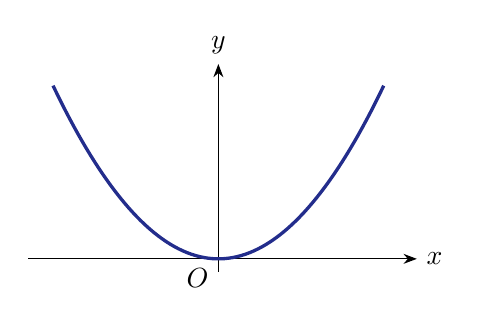
\begin{tikzpicture}[x=1.05cm,y=.55cm,>=Stealth]
 \draw[->] (-2.3,0)--(2.4,0) node[right] {$x$};
 \draw[->] (0,-.3)--(0,4.5) node[above] {$y$};
 \draw[answerblue,very thick,samples=80,domain=-2:2] plot (\x,{\x*\x});
 \node[below left] at (0,0) {$O$};
\end{tikzpicture}
\end{center}
\figtitle{Parabol $y=x^2$ đối xứng qua trục tung.}
\end{vidu}
\begin{vidu}
\vidutitle{Ví dụ 02 [TDM21].} Xét $y=f(x)=\cos x$.
Ta có $f(-x)=\cos(-x)=\cos x=f(x)$ với mọi $x\in\mathbb R$.
Suy ra $y=\cos x$ là hàm số chẵn.
\end{vidu}
\tieumuc{1.2. Hàm số lẻ}
\luuy{Hàm số $y=f(x)$ có tập xác định $D$ là \textbf{hàm số lẻ} nếu với mọi $x\in D$ thì $-x\in D$ và $f(-x)=-f(x)$.}
\luuy{Đồ thị hàm số lẻ nhận gốc tọa độ $O$ làm \textbf{tâm đối xứng}.}
\begin{vidu}
\vidutitle{Ví dụ 03 [TDM21].} Xét hàm số $y=f(x)=x$.
Có $f(-x)=-x=-f(x)$ với mọi $x\in\mathbb R$.
Suy ra $y=x$ là hàm số lẻ.
\begin{center}
\begin{tikzpicture}[scale=.8,>=Stealth]
 \draw[->] (-2.6,0)--(2.7,0) node[right] {$x$};
 \draw[->] (0,-2.2)--(0,2.3) node[above] {$y$};
 \draw[answerblue,very thick] (-2,-2)--(2,2);
 \node[below right] at (0,0) {$O$};
\end{tikzpicture}
\end{center}
\figtitle{Đường thẳng $y=x$ có tâm đối xứng $O$.}
\end{vidu}
\begin{vidu}
\vidutitle{Ví dụ 04 [TDM21].} Xét $y=f(x)=\sin x$.
Vì $f(-x)=\sin(-x)=-\sin x=-f(x)$ nên $y=\sin x$ là hàm số lẻ.
\end{vidu}
\luuy{Các hàm số $y=\sin x$, $y=\tan x$, $y=\cot x$ là \textbf{hàm số lẻ} trên tập xác định tương ứng.}
\muctieu{2. HÀM SỐ TUẦN HOÀN -- CHU KÌ $T$}
\luuy{Hàm số $y=f(x)$ là hàm \textbf{tuần hoàn với chu kì cơ bản $T$} nếu $T>0$ là số nhỏ nhất sao cho với mọi $x\in D$:
\[
x+T\in D,\qquad x-T\in D,\qquad f(x+T)=f(x).
\]}
\luuy{Khi đó $f(x+kT)=f(x)$ với mọi $x\in D$ và $k\in\mathbb Z$.}
\tieumuc{Các kết quả quan trọng}
\begin{center}
\renewcommand{\arraystretch}{1.5}
\begin{tabular}{|>{\raggedright\arraybackslash}p{.69\linewidth}|>{\centering\arraybackslash}p{.18\linewidth}|}\hline
\textbf{Hàm số} & \textbf{Chu kì}\\\hline
$y=\sin x$ và $y=\cos x$ & $2\pi$\\\hline
$y=\tan x$ và $y=\cot x$ & $\pi$\\\hline
$y=\alpha\sin(ax+b)+\beta$, $y=\alpha\cos(ax+b)+\beta$ & $\dfrac{2\pi}{|a|}$\\\hline
$y=\alpha\tan(ax+b)+\beta$, $y=\alpha\cot(ax+b)+\beta$ & $\dfrac{\pi}{|a|}$\\\hline
\end{tabular}
\end{center}
{\small\itshape Với hai dòng cuối, giả sử $\alpha\ne0$, $a\ne0$.}
\clearpage

\muctieu{3. CÁC HÀM LƯỢNG GIÁC CƠ BẢN}
\tieumuc{3.1. Hàm số $y=\sin x$}
\begin{itemize}
 \item Tập xác định: $D=\mathbb R$. Tập giá trị: $[-1;1]$ vì $-1\le\sin x\le1$.
 \item Là hàm số lẻ; đồ thị nhận $O$ làm tâm đối xứng.
 \item Tuần hoàn với chu kì $T=2\pi$.
\end{itemize}
\textbf{Sự biến thiên trên một chu kì $[-\pi;\pi]$:}
\begin{center}
\renewcommand{\arraystretch}{1.55}
\begin{tabular}{|c|c|c|c|c|c|}\hline
$x$ & $-\pi$ & $-\frac{\pi}{2}$ & $0$ & $\frac{\pi}{2}$ & $\pi$\\\hline
$\sin x$ & $0$ & $-1$ & $0$ & $1$ & $0$\\\hline
Chiều biến thiên & \multicolumn{2}{c|}{$\searrow$} & $\nearrow$ & $\nearrow$ & $\searrow$\\\hline
\end{tabular}
\end{center}
\begin{center}
\begin{tikzpicture}[x=1.3cm,y=1.2cm,>=Stealth]
 \draw[->] (-3.5,0)--(3.6,0) node[right] {$x$};
 \draw[->] (0,-1.45)--(0,1.45) node[above] {$y$};
 \draw[answerblue,thick,samples=120,domain=-3.14159:3.14159] plot (\x,{sin(\x r)});
 \foreach \x/\lab in {-3.14159/{-\pi},-1.5708/{-\frac{\pi}{2}},1.5708/{\frac{\pi}{2}},3.14159/{\pi}}{
 \draw (\x,.05)--(\x,-.05) node[below=3pt] {\scriptsize$\lab$};}
 \node[below left] at (0,0) {$O$};
 \node[left] at (0,1) {$1$};\node[left] at (0,-1) {$-1$};
 \fill[answerblue] (1.5708,1) circle (1.7pt);
 \fill[answerblue] (-1.5708,-1) circle (1.7pt);
\end{tikzpicture}\qquad
\trigcircle{\fill[answerblue] (0,1) circle (1.7pt);\fill[answerblue] (0,-1) circle (1.7pt);}
\figtitle{Đồ thị trong một chu kì và đường tròn lượng giác.}
\end{center}
\textbf{Đồ thị trên toàn $\mathbb R$:}
\begin{center}
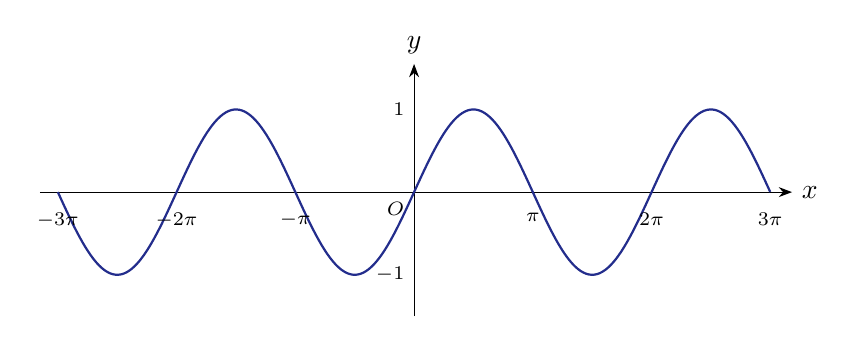
\begin{tikzpicture}[x=.48cm,y=1.05cm,>=Stealth]
 \draw[->] (-9.9,0)--(10,0) node[right] {$x$};
 \draw[->] (0,-1.5)--(0,1.55) node[above] {$y$};
 \draw[answerblue,thick,samples=260,domain=-9.42477:9.42477] plot (\x,{sin(\x r)});
 \foreach \x/\lab in {-9.42477/{-3\pi},-6.28318/{-2\pi},-3.14159/{-\pi},3.14159/{\pi},6.28318/{2\pi},9.42477/{3\pi}}{
 \node[below=4pt] at (\x,0) {\scriptsize$\lab$};}
 \node[below left] at (0,0) {\scriptsize$O$};
 \node[left] at (0,1) {\scriptsize$1$};
 \node[left] at (0,-1) {\scriptsize$-1$};
\end{tikzpicture}
\end{center}
\luuy{$y=\sin x$ \textbf{đồng biến} trên mỗi khoảng
$\left(-\frac{\pi}{2}+2k\pi\,;\,\frac{\pi}{2}+2k\pi\right)$,
\textbf{nghịch biến} trên mỗi khoảng
$\left(\frac{\pi}{2}+2k\pi\,;\,\frac{3\pi}{2}+2k\pi\right)$, $k\in\mathbb Z$.}
\begin{vidu}
\vidutitle{Ví dụ 01 [TDM31].} Khảo sát và vẽ đồ thị các hàm số:
\begin{enumerate}[label=\arabic*.,leftmargin=8mm]
 \item $y=3\sin\left(2x-\dfrac{\pi}{4}\right)$.
 \item $y=-4\sin\left(3x+\dfrac{\pi}{3}\right)$.
\end{enumerate}
{\bfseries\color{answerblue}Giải:} \textit{Để trống như tài liệu gốc.}\par\vspace{14mm}
\end{vidu}
\clearpage

\tieumuc{3.2. Hàm số $y=\cos x$}
\begin{itemize}
 \item Tập xác định: $D=\mathbb R$. Tập giá trị: $[-1;1]$ vì $-1\le\cos x\le1$.
 \item Là hàm số chẵn; đồ thị nhận $Oy$ làm trục đối xứng.
 \item Tuần hoàn với chu kì $T=2\pi$.
\end{itemize}
\textbf{Sự biến thiên trên một chu kì $[-\pi;\pi]$:}
\begin{center}
\renewcommand{\arraystretch}{1.55}
\begin{tabular}{|c|c|c|c|c|c|}\hline
$x$ & $-\pi$ & $-\frac{\pi}{2}$ & $0$ & $\frac{\pi}{2}$ & $\pi$\\\hline
$\cos x$ & $-1$ & $0$ & $1$ & $0$ & $-1$\\\hline
Chiều biến thiên & \multicolumn{2}{c|}{$\nearrow$} & $\nearrow$ & $\searrow$ & $\searrow$\\\hline
\end{tabular}
\end{center}
\begin{center}
\begin{tikzpicture}[x=1.3cm,y=1.2cm,>=Stealth]
 \draw[->] (-3.5,0)--(3.6,0) node[right] {$x$};
 \draw[->] (0,-1.45)--(0,1.45) node[above] {$y$};
 \draw[answerblue,thick,samples=120,domain=-3.14159:3.14159] plot (\x,{cos(\x r)});
 \foreach \x/\lab in {-3.14159/{-\pi},-1.5708/{-\frac{\pi}{2}},1.5708/{\frac{\pi}{2}},3.14159/{\pi}}{
 \draw (\x,.05)--(\x,-.05) node[below=3pt] {\scriptsize$\lab$};}
 \node[below left] at (0,0) {$O$};
 \node[left] at (0,1) {$1$};\node[left] at (0,-1) {$-1$};
 \fill[answerblue] (0,1) circle (1.7pt);
\end{tikzpicture}\qquad
\trigcircle{\fill[answerblue] (1,0) circle (1.7pt);\fill[answerblue] (-1,0) circle (1.7pt);}
\figtitle{Đồ thị trong một chu kì và đường tròn lượng giác.}
\end{center}
\textbf{Đồ thị trên toàn $\mathbb R$:}
\begin{center}
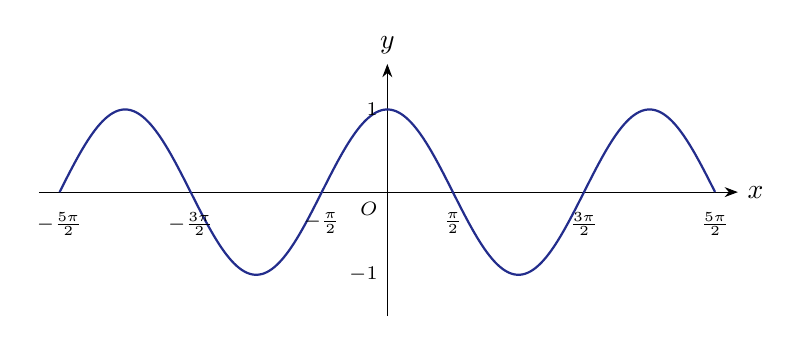
\begin{tikzpicture}[x=.53cm,y=1.05cm,>=Stealth]
 \draw[->] (-8.35,0)--(8.4,0) node[right] {$x$};
 \draw[->] (0,-1.5)--(0,1.55) node[above] {$y$};
 \draw[answerblue,thick,samples=260,domain=-7.85398:7.85398] plot (\x,{cos(\x r)});
 \foreach \x/\lab in {-7.85398/{-\frac{5\pi}{2}},-4.71239/{-\frac{3\pi}{2}},-1.5708/{-\frac{\pi}{2}},1.5708/{\frac{\pi}{2}},4.71239/{\frac{3\pi}{2}},7.85398/{\frac{5\pi}{2}}}{
 \node[below=4pt] at (\x,0) {\scriptsize$\lab$};}
 \node[below left] at (0,0) {\scriptsize$O$};
 \node[left] at (0,1) {\scriptsize$1$};
 \node[left] at (0,-1) {\scriptsize$-1$};
\end{tikzpicture}
\end{center}
\luuy{$y=\cos x$ \textbf{đồng biến} trên mỗi khoảng
$(-\pi+2k\pi\,;\,2k\pi)$,
\textbf{nghịch biến} trên mỗi khoảng $(2k\pi\,;\,\pi+2k\pi)$, $k\in\mathbb Z$.}
\begin{vidu}
\vidutitle{Ví dụ 01 [TDM32].} Khảo sát và vẽ đồ thị hàm số
\[
y=-4\cos 2x+1.
\]
{\bfseries\color{answerblue}Giải:} \textit{Để trống như tài liệu gốc.}\par\vspace{14mm}
\end{vidu}
\clearpage

\tieumuc{3.3. Hàm số $y=\tan x$}
\luuy{\textbf{Định nghĩa:} Với $x\ne\frac{\pi}{2}+k\pi$, $k\in\mathbb Z$, đặt
$\tan x=\frac{\sin x}{\cos x}$.}
\textbf{Bài toán:} Khảo sát và vẽ đồ thị hàm số $y=\tan x$.
\begin{itemize}
 \item Tập xác định:
 $D=\mathbb R\setminus\left\{\frac{\pi}{2}+k\pi\ \middle|\ k\in\mathbb Z\right\}$.
 \item Là hàm số lẻ; đồ thị nhận gốc $O$ làm tâm đối xứng.
 \item Tuần hoàn với chu kì $T=\pi$.
 \item Đồng biến trên $\left(-\frac{\pi}{2};\frac{\pi}{2}\right)$.
\end{itemize}
\textbf{Bảng biến thiên trong một chu kì:}
\begin{center}
\renewcommand{\arraystretch}{1.6}
\begin{tabular}{|c|c|c|c|}\hline
$x$ & $-\frac{\pi}{2}$ & $0$ & $\frac{\pi}{2}$\\\hline
$\tan x$ & $-\infty$ & $0$ & $+\infty$\\\hline
Biến thiên & \multicolumn{3}{c|}{$-\infty\quad\nearrow\quad 0\quad\nearrow\quad +\infty$}\\\hline
\end{tabular}
\end{center}
\begin{center}
\begin{tikzpicture}[x=1.6cm,y=.72cm,>=Stealth]
 \draw[->] (-1.85,0)--(1.92,0) node[right] {$x$};
 \draw[->] (0,-2.55)--(0,2.6) node[above] {$y$};
 \draw[dashed,gray] (-1.5708,-2.5)--(-1.5708,2.5);
 \draw[dashed,gray] (1.5708,-2.5)--(1.5708,2.5);
 \begin{scope}
  \clip (-1.75,-2.5) rectangle (1.75,2.5);
  \draw[answerblue,thick,samples=120,domain=-1.47:1.47] plot (\x,{tan(\x r)});
 \end{scope}
 \node[below right] at (0,0) {$O$};
 \node[above left] at (-1.5708,0) {$-\frac{\pi}{2}$};
 \node[above right] at (1.5708,0) {$\frac{\pi}{2}$};
\end{tikzpicture}
\figtitle{Đồ thị $y=\tan x$ trên khoảng $\left(-\pi/2;\pi/2\right)$.}
\end{center}
\textbf{Đồ thị trên toàn $\mathbb R$:}
\begin{center}
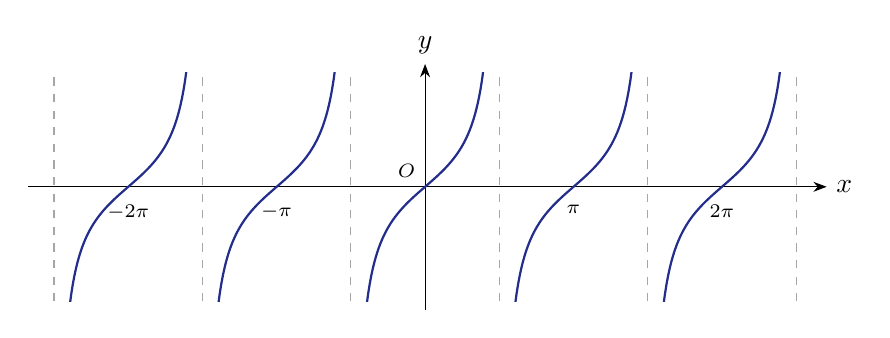
\begin{tikzpicture}[x=.6cm,y=.52cm,>=Stealth]
 \draw[->] (-8.4,0)--(8.5,0) node[right] {$x$};
 \draw[->] (0,-3)--(0,3) node[above] {$y$};
 \begin{scope}
 \clip (-8.2,-2.8) rectangle (8.2,2.8);
 \foreach \k in {-2,-1,0,1,2}{
  \pgfmathsetmacro{\a}{\k*3.14159265-1.47}
  \pgfmathsetmacro{\b}{\k*3.14159265+1.47}
  \draw[answerblue,thick,samples=90,domain=\a:\b] plot (\x,{tan(\x r)});
 }
 \end{scope}
 \foreach \k in {-2,-1,0,1,2}{
  \pgfmathsetmacro{\a}{\k*3.14159265+1.5707963}
  \draw[dashed,gray!70] (\a,-2.8)--(\a,2.8);
  \pgfmathsetmacro{\b}{\k*3.14159265-1.5707963}
  \draw[dashed,gray!70] (\b,-2.8)--(\b,2.8);
 }
 \foreach \x/\lab in {-6.28318/{-2\pi},-3.14159/{-\pi},3.14159/{\pi},6.28318/{2\pi}}{
 \node[below=3pt] at (\x,0) {\scriptsize$\lab$};}
 \node[above left] at (0,0) {\scriptsize$O$};
\end{tikzpicture}
\end{center}
\luuy{$y=\tan x$ \textbf{đồng biến} trên mỗi khoảng
$\left(-\frac{\pi}{2}+k\pi\,;\,\frac{\pi}{2}+k\pi\right)$, $k\in\mathbb Z$.}
\tieumuc{Mở rộng}
Với $y=m\tan(ax+b)+n$, $m>0,\ a>0$, hàm số đồng biến trên các khoảng
\[
-\frac{\pi}{2}+k\pi<ax+b<\frac{\pi}{2}+k\pi
\Longleftrightarrow
-\frac{\pi}{2a}-\frac ba+\frac{k\pi}{a}<x<
\frac{\pi}{2a}-\frac ba+\frac{k\pi}{a},
\quad k\in\mathbb Z.
\]
\clearpage

\tieumuc{3.4. Hàm số $y=\cot x$}
\luuy{\textbf{Định nghĩa:} Với $x\ne k\pi$, $k\in\mathbb Z$, đặt
$\cot x=\frac{\cos x}{\sin x}$.}
\textbf{Bài toán:} Khảo sát và vẽ đồ thị hàm số $y=\cot x$.
\begin{itemize}
 \item Tập xác định:
 $D=\mathbb R\setminus\{k\pi\mid k\in\mathbb Z\}$.
 \item Là hàm số lẻ; đồ thị nhận gốc $O$ làm tâm đối xứng.
 \item Tuần hoàn với chu kì $T=\pi$.
 \item Nghịch biến trên $(0;\pi)$.
\end{itemize}
\textbf{Bảng biến thiên trong một chu kì:}
\begin{center}
\renewcommand{\arraystretch}{1.6}
\begin{tabular}{|c|c|c|c|}\hline
$x$ & $0$ & $\frac{\pi}{2}$ & $\pi$\\\hline
$\cot x$ & $+\infty$ & $0$ & $-\infty$\\\hline
Biến thiên & \multicolumn{3}{c|}{$+\infty\quad\searrow\quad0\quad\searrow\quad-\infty$}\\\hline
\end{tabular}
\end{center}
\begin{center}
\begin{tikzpicture}[x=1.5cm,y=.72cm,>=Stealth]
 \draw[->] (-.3,0)--(3.45,0) node[right] {$x$};
 \draw[->] (0,-2.55)--(0,2.6) node[above] {$y$};
 \draw[dashed,gray] (3.14159,-2.5)--(3.14159,2.5);
 \begin{scope}
  \clip (-.1,-2.5) rectangle (3.3,2.5);
  \draw[answerblue,thick,samples=120,domain=.13:3.01] plot (\x,{1/tan(\x r)});
 \end{scope}
 \node[below left] at (0,0) {$O$};
 \node[below=3pt] at (1.5708,0) {$\frac{\pi}{2}$};
 \node[above right] at (3.14159,0) {$\pi$};
\end{tikzpicture}
\figtitle{Đồ thị $y=\cot x$ trên khoảng $(0;\pi)$.}
\end{center}
\textbf{Đồ thị trên toàn $\mathbb R$:}
\begin{center}
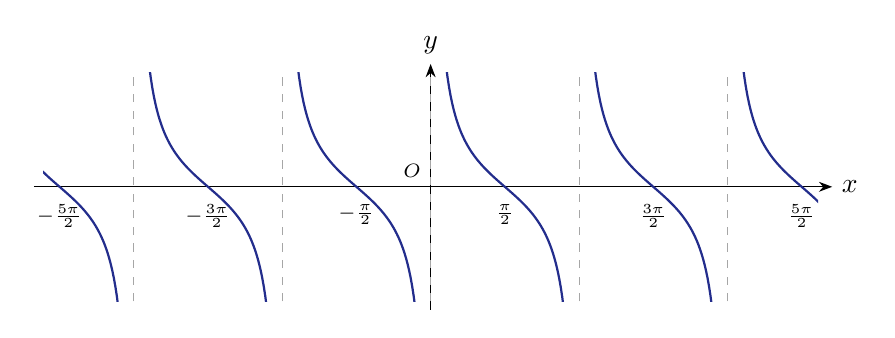
\begin{tikzpicture}[x=.6cm,y=.52cm,>=Stealth]
 \draw[->] (-8.4,0)--(8.5,0) node[right] {$x$};
 \draw[->] (0,-3)--(0,3) node[above] {$y$};
 \begin{scope}
 \clip (-8.2,-2.8) rectangle (8.2,2.8);
 \foreach \k in {-3,-2,-1,0,1,2}{
  \pgfmathsetmacro{\a}{\k*3.14159265+.13}
  \pgfmathsetmacro{\b}{(\k+1)*3.14159265-.13}
  \draw[answerblue,thick,samples=90,domain=\a:\b] plot (\x,{1/tan(\x r)});
 }
 \end{scope}
 \foreach \k in {-2,-1,0,1,2}{
  \pgfmathsetmacro{\a}{\k*3.14159265}
  \draw[dashed,gray!70] (\a,-2.8)--(\a,2.8);
 }
 \foreach \x/\lab in {-7.85398/{-\frac{5\pi}{2}},-4.71239/{-\frac{3\pi}{2}},-1.5708/{-\frac{\pi}{2}},1.5708/{\frac{\pi}{2}},4.71239/{\frac{3\pi}{2}},7.85398/{\frac{5\pi}{2}}}{
 \node[below=3pt] at (\x,0) {\scriptsize$\lab$};}
 \node[above left] at (0,0) {\scriptsize$O$};
\end{tikzpicture}
\end{center}
\luuy{$y=\cot x$ \textbf{nghịch biến} trên mỗi khoảng
$(k\pi\,;\,\pi+k\pi)$, $k\in\mathbb Z$.}
\tieumuc{Mở rộng}
Với $y=m\cot(ax+b)+n$, $m>0,\ a>0$, hàm số \textbf{nghịch biến} trên các khoảng
\[
k\pi<ax+b<\pi+k\pi
\Longleftrightarrow
-\frac ba+\frac{k\pi}{a}<x<
\frac{\pi}{a}-\frac ba+\frac{k\pi}{a},
\quad k\in\mathbb Z.
\]
\hrule\vspace{3mm}
{\small\textbf{Ghi chú biên tập:} PDF nguồn có một vài lỗi đánh máy: định nghĩa hàm lẻ ghi nhầm là hàm chẵn (trang 1), kết luận về ví dụ $y=\sin x$ ghi nhầm thành $y=x^2$ (trang 2), và phần mở rộng $y=m\cot(ax+b)+n$ ghi nhầm đồng biến thay vì nghịch biến (trang 8). Ở bản này, các lỗi đó được chỉnh theo tính chất toán học. Các bảng biến thiên đã được trình bày lại; đề ví dụ và phần giải trống được giữ theo PDF.}
\begin{center}\textbf{\color{questionpurple}---------- HẾT ----------}\end{center}
\end{document}
